
Figure~\ref{fig:joint_scores_coordinated} and 
figure~\ref{fig:joint_scores_uncoordinated} are two histograms illustrating the
distribution of joint scores achieved by the pairs in the two
treatments.  The team treatment, which in the Hallway game requires
team reasoning (because the players only succeed when they
simultaneously reach their goals), produced significantly more
successful teams.
%($p < 0.05$).\commenta{what was tested here?}
%
In particular, 19 teams (76\%) achieved a score at or above 15 points
in the team treatment, but only 3 achieved a similar score in the
individual treatment.

\begin{wraptable}{r}{0.5\textwidth}
%\begin{table}
\begin{center}
\small{
\begin{tabular}{|c|c|c|}									   
\hline
			& Individual Reasoning              & Team Reasoning 	\\ \hline
 Compete		& 32\% 					& 0\% 			\\ \hline
 Trust		& 21\% 					& 76\% 			\\ \hline
 Surrender	& 21\% 					& 8\% 			\\ \hline
 CD			& 11\% 					& 16\% 			\\ \hline
 Alternate		& 11\% 					& 0\% 			\\ \hline
 Stalemate	& 5\% 					& 0\% 			\\ \hline
\end{tabular}}
\caption{A comparison between the strategies learned by pairs in the two treatments. 
These percentages represent $19$ games in the individual reasoning experiment,
and $25$ games in the team reasoning experiment.}
\label{tab:class}
\end{center}
%\end{table}
\end{wraptable}

Table~\ref{tab:class} compares the outcomes of matches in the two
different treatments under an intuitive classification scheme, which
we based on the behavior of the participants in the final two rounds
after 18 prior rounds of learning.  We are planning much more
extensive experimentation with human participants on grid games, after
which we hope to interpret some of these classifications
(e.g., trust, CD, etc.) as types of norms.

\emph{Compete\/} means, in the final round, only one player reaches
their goal, and in the last two rounds, the players collide at least
once.  \emph{Trust\/} means both players score in the last round, but
only when one player did not take advantage of an opportunity to
defect.  \emph{Surrender\/} means that in the final two rounds, only
one player reaches the goal and does so without any collisions.
\emph{CD} (\emph{Cooperatively Defend}) means that both players score
in the final round, but each does so in a way that prevents the other
player from reaching the goal alone.  In \emph{Alternate} matches,
both players reach their goal alone exactly once in the last two
rounds, without any collisions.  Finally, in \emph{Stalemate} matches,
neither player reaches their goal in the final round.

The treatment impacts the types of behavior we observe.
The incidence of competitive behavior drops dramatically, while trust
increases threefold.  Since trust increases, surrendering becomes less
necessary, and consequently much rarer.  Also of interest, the
incidence of CD behavior doubles.  
%Perhaps people who would have engaged in competitive behavior in the individual treatment are willing to play a CD strategy in the team setting.  
%Edited 88 to 92% to correct error from chart.
Overall, 92\% of participants exhibit cooperative behavior (either
trust or CD) in the team treatment, compared to only 33\% in the
individual treatment.

%Stalemate, which  occurred only rarely even in the individual treatment, is eliminated in the team treatment.

%Table~\ref{tab:class} suggests that the team reasoning experiment encourages participants to cooperate in such a way that we can try to understand how participates find cooperative strategies given that cooperation is a shared intention,  as opposed to potentially just a personal intention.

\comment{
Figure~\ref{fig:scores_coordinated} and figure~\ref{fig:scores_uncoordinated} show plots of improving success of the matches with team-reasoning and individual reasoning respectively. Each figure contains three plots, showing results for all agents, agents which received a joint score of 10 and above and 15 and above. Each plot contains three lines showing the fraction each round ended in success, failure or a round timeout. 

All plots show an increasing measure of successful coordinations as rounds progress through each match. The plots show that the teams explicitly tasked with cooperation performed significantly better. Also, teams that scored a higher joint score converged toward optimal cooperation sooner than teams that scored lower. Teams that scored 15 points or above reached near-optimal cooperation by round 4 with both team reasoning and without, suggesting that two cooperating players needed to agree early on to achieve the best collaboration.


\begin{figure}
\centering
\begin{subfigure}{.5\textwidth}
\centering
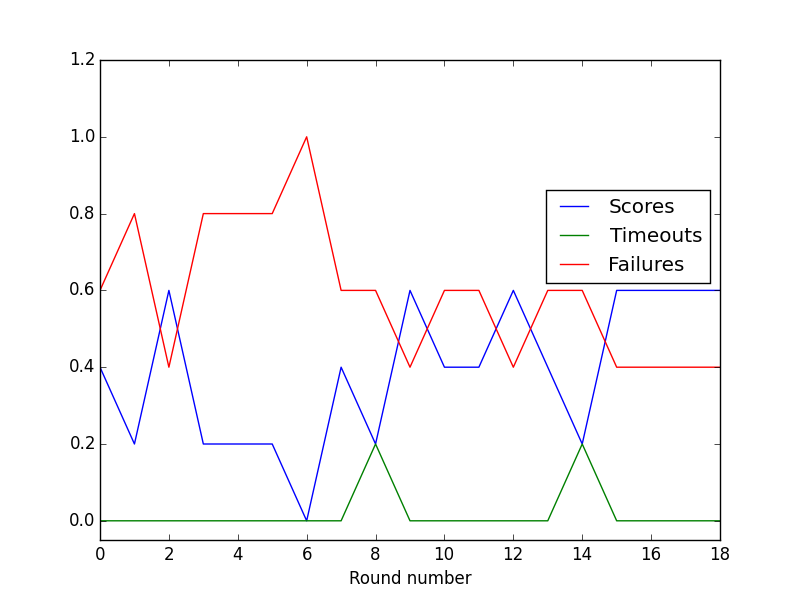
\includegraphics[width=\columnwidth]{figures/scores_coordinated_rest.png}
\caption{$< 15$ (6 teams)}
\label{fig:scores_coordinated_rest}
\end{subfigure}%
\begin{subfigure}{.5\textwidth}
\centering
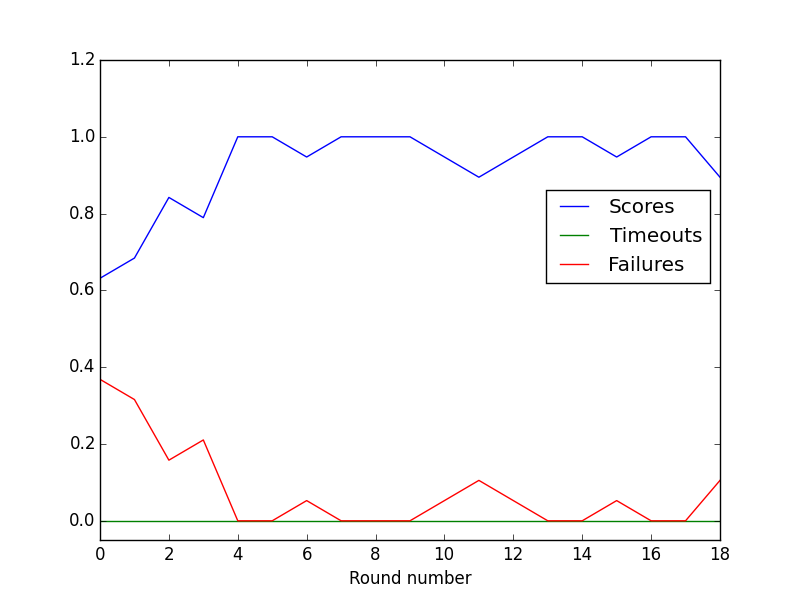
\includegraphics[width=\columnwidth]{figures/scores_coordinated_15.png}
\caption{$>= 15$ points (19 teams)}
\label{fig:scores_coordinated_15}
\end{subfigure}
\caption{Fraction of joint scores, coordination failures and round timeouts vs round number for the coordinated match group}
\label{fig:scores_coordinated}
\end{figure}

\begin{figure}
\centering
\begin{subfigure}{.5\textwidth}
\centering
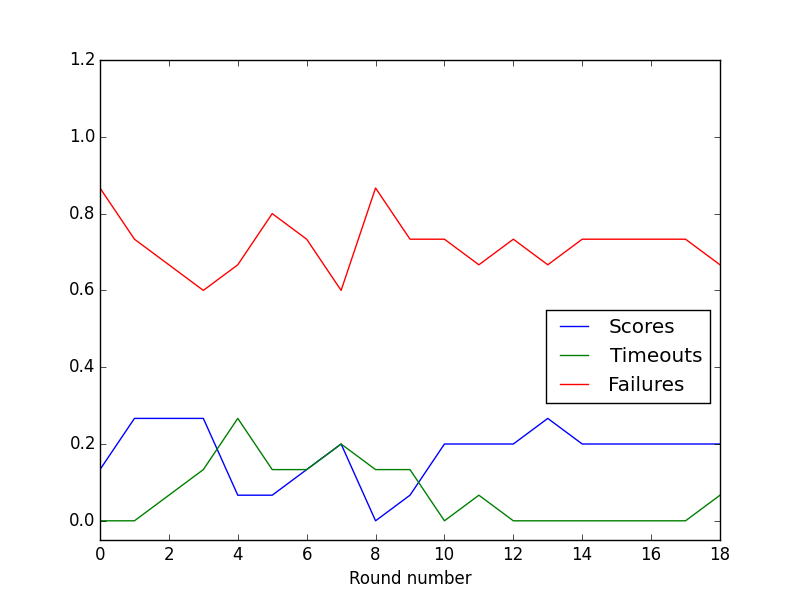
\includegraphics[width=\columnwidth]{figures/scores_uncoordinated_rest.png}
\caption{$< 15$ (17 teams)}
\label{fig:scores_uncoordinated_rest}
\end{subfigure}%
\begin{subfigure}{.5\textwidth}
\centering
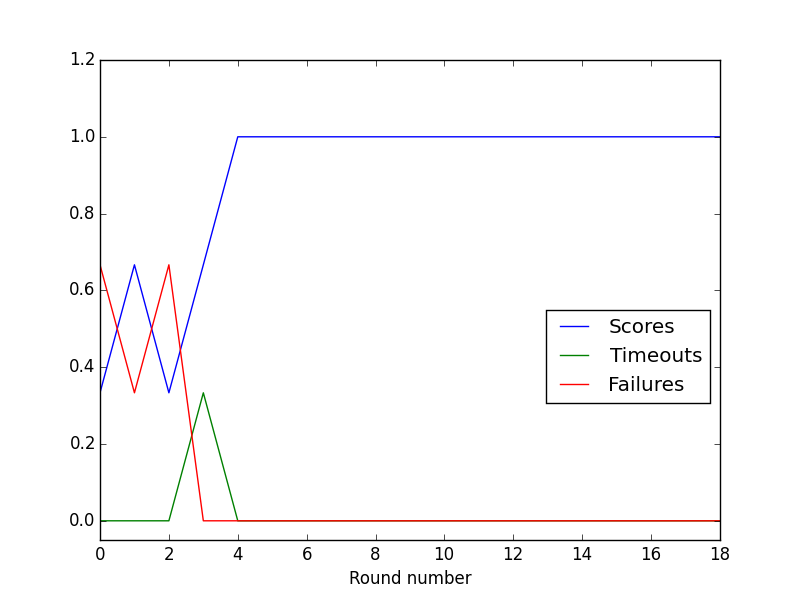
\includegraphics[width=\columnwidth]{figures/scores_uncoordinated_15.png}
\caption{$>= 15$ points (3 teams)}
\label{fig:scores_uncoordinated_15}
\end{subfigure}
\caption{Fraction of joint scores, coordination failures and round timeouts vs round number for the uncoordinated match group}
\label{fig:scores_uncoordinated}
\end{figure}


Another measure of team cooperation is the number of turns required to complete a round. Figure~\ref{fig:lengths_coordinated} and figure~\ref{fig:lengths_uncoordinated} show plots of the number of turns per round for matches with team-reasoning and with independent reasoning.

While each plot shows a lower trajectory length initially, it corresponds to lower success from figures~\ref{fig:scores_coordinated} and ~\ref{fig:scores_uncoordinated}. All matches experienced an initial increase in number of turns, but for the most cooperative teams, it quickly returns to a steady state. In the team reasoning matches, less cooperative teams experienced periodic bouts of uncoordinated rounds.

Though there were only three teams classified as cooperative in the individual reasoning group, they exhibited a more exaggerated version of the cooperative teams in the team reasoning study, suggesting that the behavior of fully cooperative teams in a more open setting will exhibit similar behaviors. For both groups of individual reasoning teams, the initial rise in the number of turns is significantly exaggerated over the team-reasoning group. 


\begin{figure}
\centering
\begin{subfigure}{.5\textwidth}
\centering
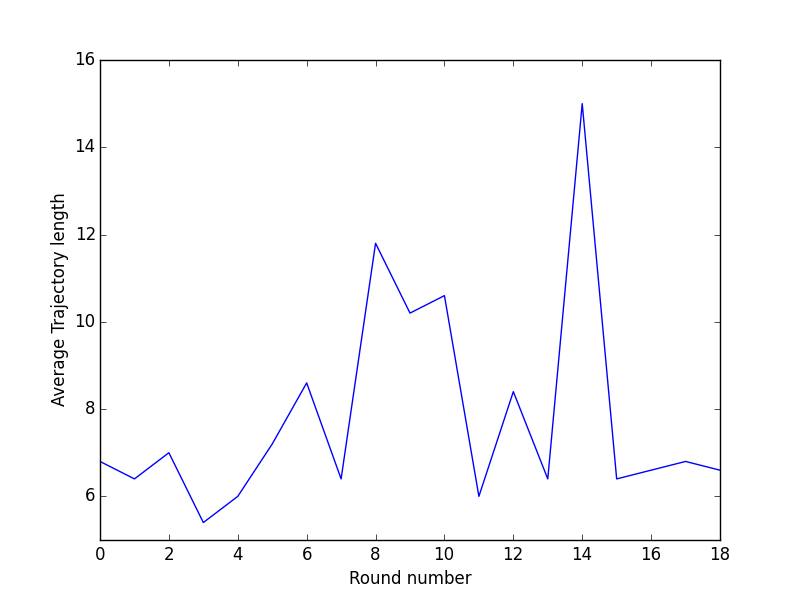
\includegraphics[width=\columnwidth]{figures/lengths_coordinated_rest.png}
\caption{$< 15$ points (6 teams)}
\label{fig:lengths_coordinated_rest}
\end{subfigure}%
\begin{subfigure}{.5\textwidth}
\centering
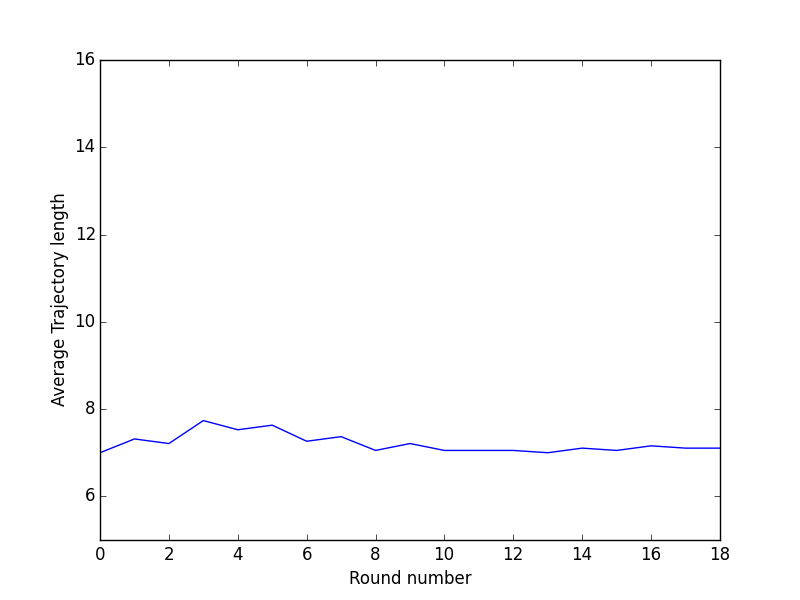
\includegraphics[width=\columnwidth]{figures/lengths_coordinated_15.png}
\caption{$>= 15$ points (19 teams)}
\label{fig:lengths_coordinated_15}
\end{subfigure}
\caption{Average number of turns per round vs round number for the team reasoning group}
\label{fig:lengths_coordinated}
\end{figure}

\begin{figure}
\centering
\begin{subfigure}{.5\textwidth}
\centering
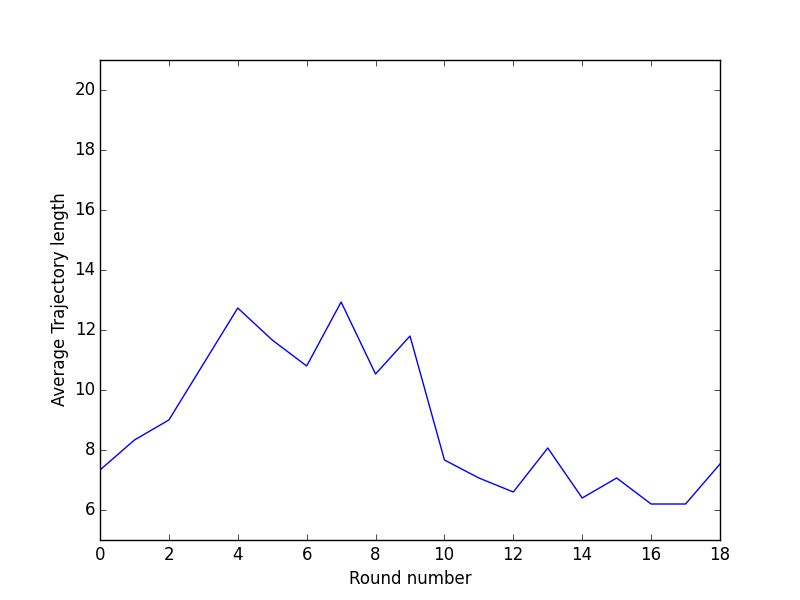
\includegraphics[width=\columnwidth]{figures/lengths_uncoordinated_rest.png}
\caption{$< 15$ points (17 teams)}
\label{fig:lengths_uncoordinated_rest}
\end{subfigure}%
\begin{subfigure}{.5\textwidth}
\centering
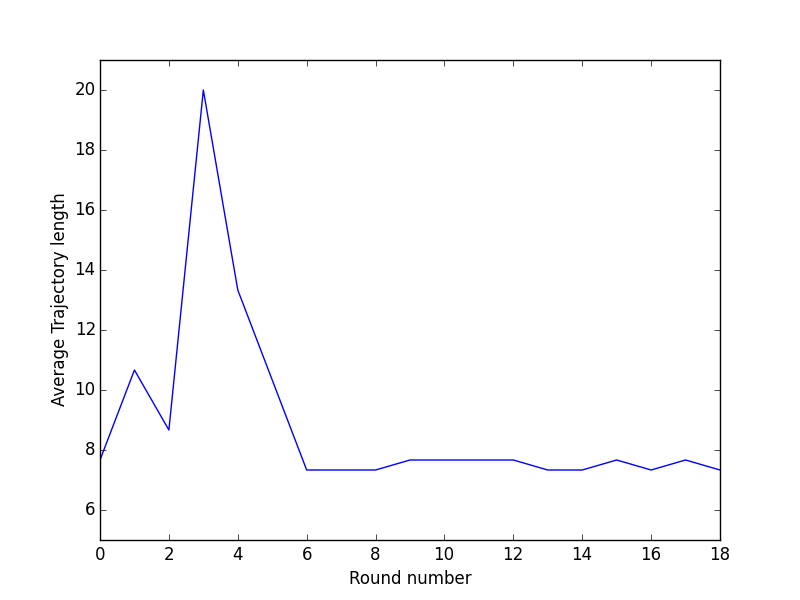
\includegraphics[width=\columnwidth]{figures/lengths_uncoordinated_15.png}
\caption{$>= 15$ points (3 teams)}
\label{fig:lengths_uncoordinated_15}
\end{subfigure}
\caption{Average number of turns per round for the individual reasoning match group}
\label{fig:lengths_uncoordinated}
\end{figure}
}

%%%subjective utility functions
The results involving human subjects playing grid games are consistent
with the results obtained in our simulations of \Q-learners playing
grid games.  In both sets of experiments, more cooperation was
achieved when the treatment incorporated social preferences.  While
the subjective utility functions of artificial agents are within our
control, so that we can perhaps lead artificial agents towards
collaborative behavior, the subjective utility functions of humans are
not.  Nonetheless, behavioral economists often infer approximations of
utility functions from experimental data by assuming some underlying
structural form, and then estimating the relevant
parameters~\cite{blanco11,fisman07}.  Likewise, one of the primary
uses of our Turk experimental framework is to generate trace data of
humans playing grid games and learning norms (such as trust, CD,
etc.), so that we can then proceed to infer utility functions and
relate them back to the norms they produce.

Next we present our proposed norm representation.  We then present an
algorithm for learning norms from trace data, human- or
machine-generated.  We also present an interactive algorithm, in which
agents can learn while at the same time establishing a norm.  We then
proceed to demonstrate the viability of our algorithms on human-human
(Turk) and agent-agent (simulation) data.  A key step in our plan for
future work is to integrate our learning algorithms with the Turk
platform, so that we can study interactive human and agent learning.

%together with an algorithm for learning norms, which, as an
%intermediate step, involves learning utility functions, which we
%ultimately do from human trace data.
